\chapter{Experimental Design and Best Practices}
\label{ch:expdesign}

\begin{sourcebox}
Statistical recommendations are assay- and objective-specific. The RNA-seq discussion uses the negative-binomial framework implemented by DESeq2 \cite{love2014}, while platform-capacity examples are independently recalculated from bases rather than inferred from a flow-cell product name.
\end{sourcebox}

\begin{keyconcept}
Experimental design is the single most important factor in determining whether a sequencing experiment will produce reliable, interpretable results. No amount of computational sophistication can compensate for a fundamentally flawed experimental design. Careful planning of replicates, sequencing depth, controls, and batch structure before the first sample is collected saves enormous time, money, and frustration.
\end{keyconcept}

\section{Why Experimental Design Matters}
\label{sec:expdesign:why}

The principle of ``garbage in, garbage out'' applies with particular force to NGS experiments. A poorly designed experiment can lead to:

\begin{itemize}[itemsep=2pt]
  \item \textbf{False discoveries:} Confounded variables produce spurious biological conclusions.
  \item \textbf{Missed discoveries:} Insufficient statistical power prevents detection of real effects.
  \item \textbf{Wasted resources:} Sequencing at the wrong depth, with too few replicates, or with inappropriate read lengths wastes budget.
  \item \textbf{Irreproducible results:} Uncontrolled batch effects and undocumented variables prevent replication.
\end{itemize}

This chapter covers the key design decisions for NGS experiments: biological versus technical replication, sequencing depth, read length, power analysis, batch effects, controls, multiplexing, sample handling, and budgeting.

%=============================================================================
\section{Biological Replicates vs Technical Replicates}
\label{sec:expdesign:replicates}
%=============================================================================

\begin{keyconcept}[title={Replicates}]
\textbf{Biological replicates} are independent biological samples---different animals, different cell culture flasks, different patients. They capture the natural biological variability in the system under study and are essential for statistical inference.

\textbf{Technical replicates} are repeated measurements of the same biological sample---the same RNA extraction sequenced twice, or the same library loaded on two lanes. They capture measurement variability but do not capture biological variability.
\end{keyconcept}

For most NGS applications, \textbf{biological replicates are far more important than technical replicates}. Modern sequencing platforms have sufficiently low technical variability that technical replication adds little value. Investment in additional biological replicates almost always provides more statistical power than technical replicates.

\begin{warningbox}[title={Common Mistake: Pseudoreplication}]
Pseudoreplication occurs when non-independent samples are treated as independent replicates. Examples include: (1) sequencing three aliquots of the same RNA extraction and calling them ``triplicates,'' (2) treating individual cells from the same animal as biological replicates in a single-cell experiment, or (3) splitting a single library across three lanes and treating the results as replicates. Pseudoreplication inflates statistical significance and produces unreliable results.
\end{warningbox}

\subsection{Minimum Replicates by Assay Type}

The number of replicates required depends on the assay, the effect size you expect to detect, and the variability of your biological system. The following guidelines represent community consensus:

\begin{table}[htbp]
\centering
\caption{Recommended minimum biological replicates by assay type.}
\label{tab:min-replicates}
\small
\renewcommand{\arraystretch}{1.3}
\begin{tabularx}{\textwidth}{@{}l c X@{}}
\toprule
\textbf{Assay} & \textbf{Min Replicates} & \textbf{Notes} \\
\midrule
RNA-seq (differential expression) & 3 (5+ recommended) & 3 is the bare minimum; 5+ replicates per condition recommended for detecting moderate fold changes ($<$2-fold). With 3 replicates, only large effects are detectable. \\
\addlinespace
ChIP-seq & 2 & ENCODE standard: 2 biological replicates per condition. Consistency measured by IDR (Irreproducible Discovery Rate). \\
\addlinespace
ATAC-seq & 2+ & 2 minimum; 3+ recommended for differential accessibility analysis. \\
\addlinespace
WGS (germline) & 1 per individual & Each individual is its own biological unit. No replication needed per individual. \\
\addlinespace
WGS (somatic/cancer) & 1 tumor + 1 normal & Matched tumor-normal pairs from the same patient. \\
\addlinespace
scRNA-seq & 2+ per condition & Biological replicates = independent samples (different animals/donors). Cells within a sample are NOT replicates. \\
\addlinespace
WGBS & 2--3 & At least 2 per condition for DMR calling. \\
\addlinespace
Hi-C & 1--2 & Deeply sequenced; replicates improve TAD boundary resolution. \\
\addlinespace
16S amplicon & 5--10+ & High variability in microbiome studies demands more replicates. \\
\bottomrule
\end{tabularx}
\end{table}

\begin{tipbox}[title={More Replicates Are Always Better}]
If your budget allows, add more biological replicates rather than increasing sequencing depth beyond the recommended minimum. A study with 3 replicates at 50M reads each will almost always outperform a study with 2 replicates at 100M reads each for detecting differentially expressed genes.
\end{tipbox}

%=============================================================================
\section{Sequencing Depth Guidelines}
\label{sec:expdesign:depth}
%=============================================================================

Sequencing depth (the number of reads or coverage) must be matched to the application. Insufficient depth leads to incomplete data; excessive depth wastes resources with diminishing returns.

\small
\renewcommand{\arraystretch}{1.3}
\begin{longtable}{@{}p{3.4cm} p{4.4cm} p{6.0cm}@{}}
\caption{Illustrative sequencing-depth starting points by application; optimal depth is study- and platform-dependent.}
\label{tab:seq-depth}\\
\toprule
\textbf{Application} & \textbf{Recommended Depth} & \textbf{Notes} \\
\midrule
\endfirsthead
\caption[]{Illustrative sequencing-depth starting points by application (continued).}\\
\toprule
\textbf{Application} & \textbf{Recommended Depth} & \textbf{Notes} \\
\midrule
\endhead
\midrule
\multicolumn{3}{r}{\textit{Continued on next page}} \\
\endfoot
\bottomrule
\endlastfoot
WGS (germline, human) & 30$\times$ coverage & Standard for clinical and research germline calling. Higher (40--60$\times$) for rare variant detection or structural variant analysis. \\
\addlinespace
WGS (somatic, tumor) & 60--100$\times$ tumor, 30--40$\times$ normal & Higher tumor depth needed to detect low-frequency somatic mutations. Ultra-deep ($>$200$\times$) for cfDNA/liquid biopsy. \\
\addlinespace
WES (exome) & 100--200$\times$ on target & Actual unique coverage depends on enrichment uniformity. \\
\addlinespace
RNA-seq (differential expression) & 20--30M read pairs & Sufficient for robust differential expression of medium-to-high expressed genes. \\
\addlinespace
RNA-seq (isoform/transcript discovery) & 50--100M read pairs & Deeper sequencing needed to detect lowly expressed isoforms and novel transcripts. \\
\addlinespace
scRNA-seq (10x Chromium) & 20,000--50,000 reads per cell & Trade-off: more cells at lower depth vs fewer cells at higher depth. For most applications, more cells is preferred. Minimum 5,000 cells per sample recommended. \\
\addlinespace
ATAC-seq & 50--75M unique fragments per replicate & After filtering (mitochondrial, duplicates), expect 25--50M usable fragments. Paired-end sequencing required. \\
\addlinespace
ChIP-seq (sharp marks) & 20--40M reads & For transcription factors and H3K4me3. ENCODE recommends 20M usable reads minimum. \\
\addlinespace
ChIP-seq (broad marks) & 40--60M reads & For H3K27me3, H3K36me3, H3K9me3. Broader domains require more reads to resolve. \\
\addlinespace
CUT\&Tag & 3--8M reads & CUT\&Tag has much lower background than ChIP-seq, requiring far fewer reads. \\
\addlinespace
Hi-C & Resolution-dependent & 1--2 billion read pairs for 1\kilobase{} resolution; 200--400M for 10\kilobase{} resolution; 50--100M for TAD identification. \\
\addlinespace
WGBS & 10--30$\times$ genome coverage & 10$\times$ minimum for CpG methylation calls; 30$\times$ for confident non-CpG methylation. \\
\addlinespace
RRBS & 10--30M reads & Reduced representation targets CpG-rich regions. \\
\addlinespace
16S amplicon & 10,000--100,000 reads/sample & 10,000 minimum for community surveys; 50,000+ for rare taxon detection. \\
\addlinespace
Shotgun metagenomics & 5--20M reads/sample & More for strain-level resolution or metagenomic assembly. \\
\end{longtable}

\begin{warningbox}[title={Depth vs Coverage vs Reads}]
These terms are often used interchangeably but have distinct meanings:
\begin{itemize}[nosep]
  \item \textbf{Reads:} The total number of sequencing reads generated (e.g., 30 million).
  \item \textbf{Coverage (fold coverage):} The average number of times each base in the target region is sequenced. For WGS: coverage $\approx$ (number of reads $\times$ read length) / genome size.
  \item \textbf{Depth:} Typically synonymous with coverage, but sometimes used to refer to the number of reads at a specific position.
\end{itemize}
Always specify whether you mean total reads, uniquely mapped reads, or fold coverage, as the distinction matters for experimental planning.
\end{warningbox}

%=============================================================================
\section{Read Length Considerations}
\label{sec:expdesign:readlength}
%=============================================================================

The choice of read length and single-end (SE) versus paired-end (PE) sequencing depends on the application:

\begin{table}[htbp]
\centering
\caption{Read length recommendations by application.}
\label{tab:read-length}
\small
\renewcommand{\arraystretch}{1.3}
\begin{tabularx}{\textwidth}{@{}l l X@{}}
\toprule
\textbf{Application} & \textbf{Recommended} & \textbf{Rationale} \\
\midrule
WGS & PE 150\basepair & Standard; good balance of mappability and throughput. \\
WES & PE 75--150\basepair & PE 100 or PE 150 both work well. \\
RNA-seq (DE) & PE 75--100\basepair & Sufficient for gene-level quantification. Longer reads provide marginal benefit for DE. \\
RNA-seq (isoforms) & PE 150\basepair & Longer reads improve splice junction detection and transcript assembly. \\
scRNA-seq (10x 3') & SE 28 + SE 91 (or SE 150) & R1 is barcode+UMI (28\basepair); R2 is cDNA. SE 91 sufficient for gene counting. \\
ATAC-seq & PE 50--75\basepair & Short PE reads are sufficient since fragments are short. PE required for fragment size analysis. \\
ChIP-seq & SE 50--75\basepair or PE 75\basepair & SE 50 is cost-effective for peak calling. PE improves duplicate detection. \\
CUT\&Tag & PE 50\basepair & Short PE reads; fragments are typically $<$500\basepair. \\
Hi-C & PE 50--150\basepair & PE 50 minimizes chimeric-read artefacts; PE 150 better for long-range interactions. \\
WGBS & PE 100--150\basepair & Longer reads improve mapping of bisulfite-converted reads. \\
16S amplicon & PE 250--300\basepair & Reads must overlap to span the full amplicon (e.g., V3--V4 $\approx$460\basepair). \\
\bottomrule
\end{tabularx}
\end{table}

\begin{keyconcept}[title={Paired-End vs Single-End}]
\textbf{Paired-end (PE)} sequencing reads both ends of each fragment, providing information about fragment size (insert size) and improving read mapping, especially in repetitive regions. PE is required for applications that rely on fragment size information (ATAC-seq, Hi-C) and strongly recommended for WGS and RNA-seq.

\textbf{Single-end (SE)} sequencing reads only one end, halving the data volume but losing fragment size information. SE is acceptable for ChIP-seq peak calling and some scRNA-seq protocols where the second read is short (barcode/UMI only).
\end{keyconcept}

%=============================================================================
\section{Power Analysis}
\label{sec:expdesign:power}
%=============================================================================

Power analysis estimates the number of replicates and sequencing depth needed to detect effects of a given size with a specified confidence level. It should be performed \textit{before} the experiment to ensure adequate statistical power.

\subsection{RNA-seq Power Analysis}

\begin{description}[style=nextline, font=\bfseries, itemsep=3pt]
  \item[RNASeqPower (Bioconductor)]
  Estimates power for detecting differential expression as a function of depth, coefficient of variation (CV), fold change, sample size, and significance level. Based on the negative binomial model used by DESeq2/edgeR.

  \item[powsimR]
  A simulation-based power analysis tool that can model realistic RNA-seq data characteristics including mean-variance relationships, dropout, and multiple testing correction.

  \item[how\_many\_cells]
  Specifically designed for scRNA-seq power analysis: estimates the number of cells needed to detect a cell type or state of a given frequency in the population.
\end{description}

\begin{lstlisting}[language=R,caption={Power analysis for RNA-seq with RNASeqPower.},label=lst:power-rnaseq]
library(RNASeqPower)

# How many replicates do I need?
# Parameters: 30M reads, CV=0.4, effect=2-fold, alpha=0.05
rnapower(depth = 30, cv = 0.4, effect = 2, alpha = 0.05, power = 0.8)
# Returns: n = 3.2 -> need at least 4 replicates per condition

# Power at different replicate numbers
for (n in 2:8) {
  pwr <- rnapower(depth = 30, cv = 0.4, effect = 2, alpha = 0.05, n = n)
  cat(sprintf("n=%d: power=%.2f\n", n, pwr))
}
# Typical output:
# n=2: power=0.49
# n=3: power=0.73
# n=4: power=0.86
# n=5: power=0.92
# n=6: power=0.96
\end{lstlisting}

\begin{tipbox}[title={The Depth vs Replicates Trade-Off}]
For a fixed budget, how should you allocate resources between sequencing depth and replicates? Research consistently shows that \textbf{adding replicates provides more power than adding depth} once a minimum depth threshold is reached (approximately 10--15M reads for RNA-seq). Sequencing 3 replicates at 30M reads each is far more powerful than sequencing 2 replicates at 45M reads each. Prioritize replicates over depth.
\end{tipbox}

\subsection{Formal Power Analysis for Differential Expression}
\label{subsec:expdesign:formalpower}

Power for detecting differential expression in RNA-seq depends on five key parameters: sample size $n$ per group, effect size $\delta$ (log$_2$ fold change), biological coefficient of variation $\phi$ (dispersion), sequencing depth $d$ (in millions of reads), and significance threshold $\alpha$. Under the negative binomial model used by \software{DESeq2} and \software{edgeR}, the approximate power for a single gene is:

\begin{equation}
\label{eq:rnaseqpower}
\text{Power} = \Phi\left( \frac{|\delta| \sqrt{n / (1/\mu + \phi)}}{\sigma_\delta} - z_{1-\alpha/2} \right)
\end{equation}

where $\Phi$ is the standard normal CDF, $\mu$ is the mean expression (proportional to depth $d$), $\phi$ is the dispersion parameter (related to the coefficient of variation by $\text{CV}^2 = 1/\mu + \phi$), and $z_{1-\alpha/2}$ is the critical value. As depth $d$ increases, $1/\mu$ becomes negligible and the variance is dominated by $\phi$, the biological variability. This is why increasing replicates (which reduces the effective variance by $1/n$) is more effective than increasing depth once $\mu$ is large.

\begin{lstlisting}[language=R,caption={Formal power analysis with power curves.},label=lst:power-curves]
library(RNASeqPower)

# Power as a function of sample size for different effect sizes
sample_sizes <- 2:12
cv <- 0.4  # Biological CV (typical for human tissue)
depth <- 20  # Millions of reads (mapped)

# Generate power curves
par(mar = c(4, 4, 2, 1))
plot(NA, xlim = c(2, 12), ylim = c(0, 1),
     xlab = "Replicates per group (n)",
     ylab = "Power",
     main = "RNA-seq Power Analysis")
abline(h = 0.8, lty = 2, col = "gray")

effects <- c(1.5, 2.0, 2.5, 3.0)  # Fold changes
cols <- c("red", "blue", "darkgreen", "purple")

for (i in seq_along(effects)) {
  powers <- sapply(sample_sizes, function(n) {
    rnapower(depth = depth, cv = cv, effect = effects[i],
             alpha = 0.05, n = n)
  })
  lines(sample_sizes, powers, col = cols[i], lwd = 2)
}

legend("bottomright", legend = paste0(effects, "-fold"),
       col = cols, lwd = 2, title = "Effect size")
\end{lstlisting}

\begin{keyconcept}[title={Interpreting Power Curves}]
Power curves reveal several important patterns:
\begin{itemize}[nosep]
  \item For 2-fold changes (common in biology), at least 5--6 replicates per group are needed to reach 80\% power with $\text{CV} = 0.4$.
  \item For small effects ($<$1.5-fold), even 10+ replicates may provide insufficient power---consider whether the biological question is realistic.
  \item Diminishing returns set in beyond $\sim$8 replicates; the power gain from replicate 9 to 10 is much smaller than from replicate 3 to 4.
  \item Reducing CV (by using more homogeneous samples, e.g., cell lines vs primary tissue) dramatically increases power at every sample size.
\end{itemize}
\end{keyconcept}

\subsection{The Benjamini-Hochberg Procedure}
\label{subsec:expdesign:bh}

When testing thousands of genes simultaneously, the multiple testing problem must be addressed. The \textbf{Benjamini-Hochberg (BH) procedure} controls the \textbf{false discovery rate} (FDR)---the expected proportion of false positives among all rejected hypotheses.

\begin{protocolbox}[title={Benjamini-Hochberg Step-by-Step}]
Given $m$ hypothesis tests with p-values $p_1, p_2, \ldots, p_m$:
\begin{enumerate}[itemsep=3pt]
  \item \textbf{Sort} the p-values: $p_{(1)} \leq p_{(2)} \leq \cdots \leq p_{(m)}$.
  \item \textbf{Find the largest} $k$ such that $p_{(k)} \leq \frac{k}{m} \cdot \alpha$, where $\alpha$ is the desired FDR level (typically 0.05).
  \item \textbf{Reject} all hypotheses $H_{(1)}, H_{(2)}, \ldots, H_{(k)}$ (i.e., all hypotheses with $p \leq p_{(k)}$).
\end{enumerate}
\end{protocolbox}

The BH procedure guarantees that the FDR is controlled at level $\alpha$ when the tests are independent or positively dependent. In \software{DESeq2}, the \texttt{padj} column contains BH-adjusted p-values (also called q-values).

\begin{table}[htbp]
\centering
\caption{Comparison of multiple testing correction methods.}
\label{tab:multiple-testing}
\small
\renewcommand{\arraystretch}{1.3}
\begin{tabularx}{\textwidth}{@{}l l l X@{}}
\toprule
\textbf{Method} & \textbf{Controls} & \textbf{Stringency} & \textbf{When to Use} \\
\midrule
Bonferroni & FWER & Most conservative & Few tests; when any false positive is unacceptable (e.g., clinical validation of specific variants) \\
\addlinespace
Benjamini-Hochberg & FDR & Moderate & Standard for genome-wide discovery (DE genes, peaks, DMRs); accepts some false positives in exchange for greater sensitivity \\
\addlinespace
Storey q-value & FDR & Less conservative & Estimates $\pi_0$ (proportion of true nulls) for higher power; used by \software{qvalue} R package \\
\addlinespace
Independent Hypothesis Weighting (IHW) & FDR & Adaptive & Weights hypotheses by an independent covariate (e.g., mean expression); can increase power for RNA-seq \\
\bottomrule
\end{tabularx}
\end{table}

\begin{warningbox}[title={Bonferroni vs BH: When It Matters}]
With $m = 20{,}000$ genes tested at $\alpha = 0.05$: Bonferroni requires $p < 0.05 / 20{,}000 = 2.5 \times 10^{-6}$ to reject, while BH can reject genes with much larger p-values as long as they fall below the BH threshold line. In a typical RNA-seq experiment, Bonferroni might find 50 DE genes while BH finds 500. For discovery-oriented research, BH is almost always the appropriate choice.
\end{warningbox}

\subsection{Pilot Study Design}
\label{subsec:expdesign:pilot}

A pilot study is a small preliminary experiment designed to estimate key parameters (biological variability, effect sizes) needed to power the full study.

\begin{protocolbox}[title={Designing a Pilot Study}]
\begin{enumerate}[itemsep=3pt]
  \item \textbf{Determine the goal:} Estimate the biological coefficient of variation ($\phi$) and approximate effect sizes for your system.
  \item \textbf{Sample size:} Use 3--5 biological replicates per group. Fewer than 3 gives unreliable variance estimates; more than 5 is wasteful for a pilot.
  \item \textbf{Sequencing depth:} Use the target depth for the full study (e.g., 20--30M reads for RNA-seq) to get realistic quality metrics.
  \item \textbf{Process identically:} Use the same library preparation, sequencing platform, and bioinformatics pipeline planned for the full study.
  \item \textbf{Estimate parameters:} From pilot data, estimate per-gene dispersion ($\phi$) using \software{DESeq2} or \software{edgeR}, and compute the distribution of observed fold changes.
  \item \textbf{Power the full study:} Use the estimated $\phi$ and desired effect size in the \texttt{RNASeqPower} formula (\cref{eq:rnaseqpower}) to determine the required sample size for the main experiment.
\end{enumerate}
\end{protocolbox}

\begin{lstlisting}[language=R,caption={Using pilot data to estimate dispersion and power the full study.},label=lst:pilot-power]
library(DESeq2)
library(RNASeqPower)

# Analyse pilot data (3 vs 3, treated vs control)
pilot_dds <- DESeqDataSetFromMatrix(
  countData = pilot_counts, colData = pilot_meta,
  design = ~ condition)
pilot_dds <- DESeq(pilot_dds)

# Extract median dispersion (biological CV^2 approximation)
dispersions <- dispersions(pilot_dds)
median_disp <- median(dispersions, na.rm = TRUE)
estimated_cv <- sqrt(median_disp)
cat("Estimated biological CV:", round(estimated_cv, 2), "\n")

# Power analysis for full study using pilot estimates
for (n in c(3, 5, 7, 10, 12)) {
  pwr <- rnapower(depth = 20, cv = estimated_cv,
                   effect = 2, alpha = 0.05, n = n)
  cat(sprintf("n=%2d per group: power = %.2f\n", n, pwr))
}
\end{lstlisting}

\begin{warningbox}[title={Common Pilot Study Mistakes}]
\begin{itemize}[nosep]
  \item \textbf{Too few replicates:} With only 2 per group, variance estimates are extremely noisy, leading to unreliable power calculations.
  \item \textbf{Incorporating pilot data into the main study:} If the pilot reveals issues (contamination, unexpected batch effects, protocol changes), the pilot data may not be combinable with the main study. Decide in advance whether pilot samples will be included.
  \item \textbf{Ignoring the pilot results:} Some researchers run a pilot but proceed with the planned sample size regardless. If the pilot reveals higher-than-expected variability, increase the sample size.
  \item \textbf{Different protocols:} A pilot run with a different library prep kit, extraction method, or sequencing platform provides misleading variance estimates.
\end{itemize}
\end{warningbox}

\subsection{Cost-Optimisation Model}
\label{subsec:expdesign:costmodel}

For a fixed total budget $B$, the key trade-off in RNA-seq experimental design is between the number of samples $n$ and the sequencing depth per sample $d$. The total cost can be modelled as:

\begin{equation}
\label{eq:budget}
B = n \cdot \left( C_{\text{lib}} + d \cdot C_{\text{seq}} \right)
\end{equation}

where $C_{\text{lib}}$ is the per-sample library preparation cost (typically \$50--200), $d$ is the sequencing depth in millions of reads, and $C_{\text{seq}}$ is the cost per million reads (typically \$1--5 depending on the platform and throughput).

Solving for $n$ at a given depth:

\begin{equation}
n = \frac{B}{C_{\text{lib}} + d \cdot C_{\text{seq}}}
\end{equation}

\begin{lstlisting}[language=R,caption={Cost-optimisation: finding the optimal allocation of budget to samples vs depth.},label=lst:cost-optimise]
library(RNASeqPower)

# Budget parameters
budget <- 10000    # Total budget in USD
C_lib  <- 150      # Library prep cost per sample
C_seq  <- 3        # Cost per million reads

# Scan different depths to find optimal allocation
depths <- seq(5, 60, by = 1)
cv <- 0.4; effect <- 2; alpha <- 0.05

results <- data.frame(depth = depths, n = NA, power = NA)

for (i in seq_along(depths)) {
  d <- depths[i]
  n <- floor(budget / (C_lib + d * C_seq) / 2)  # per group
  if (n < 2) next
  pwr <- rnapower(depth = d, cv = cv, effect = effect,
                   alpha = alpha, n = n)
  results$n[i] <- n
  results$power[i] <- pwr
}

# Find optimal depth
best <- results[which.max(results$power), ]
cat(sprintf("Optimal: depth=%dM, n=%d per group, power=%.2f\n",
            best$depth, best$n, best$power))

# Plot the trade-off
plot(results$depth, results$power, type = "l", lwd = 2,
     xlab = "Depth (millions of reads)",
     ylab = "Power",
     main = sprintf("Budget = $%d: Samples vs Depth Trade-off", budget))
abline(v = best$depth, lty = 2, col = "red")
text(best$depth + 2, best$power, sprintf("n=%d/group", best$n),
     col = "red", adj = 0)
\end{lstlisting}

\begin{keyconcept}[title={The Cost-Optimisation Principle}]
For differential expression studies, the optimal budget allocation almost always favours more replicates at moderate depth over fewer replicates at high depth. This is because:
\begin{enumerate}[nosep]
  \item Statistical power depends on $n$ (through the $\sqrt{n}$ term in the test statistic), but only weakly on depth once a threshold is reached.
  \item Biological variance ($\phi$) dominates technical variance ($1/\mu$) at moderate sequencing depths ($>$10--15M reads for RNA-seq).
  \item The marginal cost of adding depth increases linearly, while the marginal power gain diminishes rapidly.
\end{enumerate}
A typical optimum for RNA-seq with a \$10,000 budget is 8--10 replicates per group at 15--20M reads, rather than 4 replicates at 40M reads.
\end{keyconcept}

%=============================================================================
\section{Batch Effects}
\label{sec:expdesign:batch}
%=============================================================================

Batch effects are systematic, non-biological variations introduced by technical factors during sample processing. They are one of the most common and insidious problems in NGS experiments.

\subsection{Common Sources of Batch Effects}

\begin{itemize}[itemsep=2pt]
  \item \textbf{Different processing days:} Samples processed on Monday vs Friday may differ systematically.
  \item \textbf{Different operators:} Variation in technique between lab members.
  \item \textbf{Different reagent lots:} Enzyme, buffer, or kit lot-to-lot variation.
  \item \textbf{Different flow cells / lanes:} Sequencing run-to-run variation.
  \item \textbf{Different library preparation batches:} The most common source of batch effects.
  \item \textbf{Different sample storage conditions:} Fresh vs frozen, different storage durations.
  \item \textbf{Different extraction methods:} Changing protocols mid-experiment.
\end{itemize}

\subsection{How to Minimize Batch Effects}

\begin{protocolbox}[title={Batch Effect Prevention Strategy}]
\begin{enumerate}[itemsep=3pt]
  \item \textbf{Process all samples simultaneously} whenever possible. If not possible, distribute conditions evenly across batches.
  \item \textbf{Randomize} sample assignment to library preparation batches, flow cell lanes, and sequencing runs.
  \item \textbf{Never confound batch with biological condition.} If all treated samples are processed in batch 1 and all controls in batch 2, batch and condition effects are indistinguishable. This is the cardinal sin of experimental design.
  \item \textbf{Use the same operator, reagent lots, and protocol} throughout the experiment.
  \item \textbf{Include reference samples} across batches to quantify and correct batch effects.
  \item \textbf{Record metadata:} Date of processing, operator, reagent lot, flow cell ID, lane. You cannot correct for batch effects you did not record.
\end{enumerate}
\end{protocolbox}

\begin{figure}[htbp]
\centering
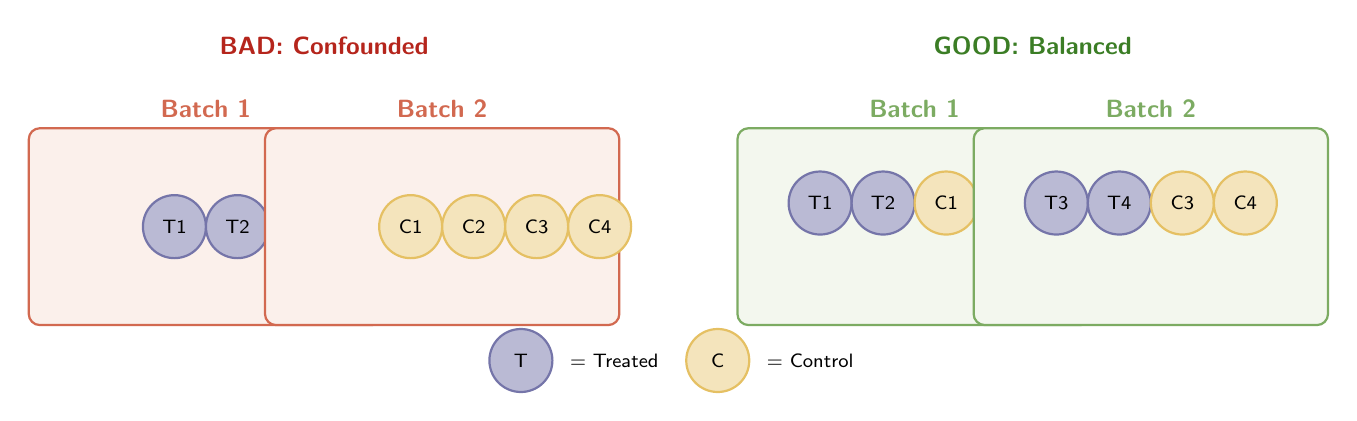
\begin{tikzpicture}[
  sample/.style={circle, draw, minimum size=0.8cm, font=\scriptsize\sffamily, thick},
  batch/.style={rectangle, draw, rounded corners=4pt, minimum width=4.5cm, minimum height=2.5cm, thick},
  label/.style={font=\small\sffamily\bfseries}
]

% BAD design
\node[label, BrickRed] at (-4.5, 3.5) {BAD: Confounded};
\node[batch, draw=BrickRed!60, fill=BrickRed!5] (b1bad) at (-6, 1.2) {};
\node[label, BrickRed!60, above] at (b1bad.north) {Batch 1};
\foreach \i in {1,...,4} {
  \node[sample, fill=MidnightBlue!30, draw=MidnightBlue!60] at (-7.2+\i*0.8, 1.2) {T\i};
}

\node[batch, draw=BrickRed!60, fill=BrickRed!5] (b2bad) at (-3, 1.2) {};
\node[label, BrickRed!60, above] at (b2bad.north) {Batch 2};
\foreach \i in {1,...,4} {
  \node[sample, fill=Goldenrod!30, draw=Goldenrod!70] at (-4.2+\i*0.8, 1.2) {C\i};
}

% GOOD design
\node[label, OliveGreen] at (4.5, 3.5) {GOOD: Balanced};
\node[batch, draw=OliveGreen!60, fill=OliveGreen!5] (b1good) at (3, 1.2) {};
\node[label, OliveGreen!60, above] at (b1good.north) {Batch 1};
\node[sample, fill=MidnightBlue!30, draw=MidnightBlue!60] at (1.8, 1.5) {T1};
\node[sample, fill=MidnightBlue!30, draw=MidnightBlue!60] at (2.6, 1.5) {T2};
\node[sample, fill=Goldenrod!30, draw=Goldenrod!70] at (3.4, 1.5) {C1};
\node[sample, fill=Goldenrod!30, draw=Goldenrod!70] at (4.2, 1.5) {C2};

\node[batch, draw=OliveGreen!60, fill=OliveGreen!5] (b2good) at (6, 1.2) {};
\node[label, OliveGreen!60, above] at (b2good.north) {Batch 2};
\node[sample, fill=MidnightBlue!30, draw=MidnightBlue!60] at (4.8, 1.5) {T3};
\node[sample, fill=MidnightBlue!30, draw=MidnightBlue!60] at (5.6, 1.5) {T4};
\node[sample, fill=Goldenrod!30, draw=Goldenrod!70] at (6.4, 1.5) {C3};
\node[sample, fill=Goldenrod!30, draw=Goldenrod!70] at (7.2, 1.5) {C4};

% Legend
\node[sample, fill=MidnightBlue!30, draw=MidnightBlue!60] at (-2, -0.5) {T};
\node[font=\scriptsize\sffamily, right] at (-1.5, -0.5) {= Treated};
\node[sample, fill=Goldenrod!30, draw=Goldenrod!70] at (0.5, -0.5) {C};
\node[font=\scriptsize\sffamily, right] at (1.0, -0.5) {= Control};

\end{tikzpicture}
\caption[Balanced batch design.]{Left: a confounded design where batch and condition are indistinguishable. Right: a balanced design where both conditions are represented in every batch. The balanced design allows batch effects to be estimated and removed computationally.}
\label{fig:batch-design}
\end{figure}

\subsection{Computational Batch Effect Correction}

When batch effects cannot be completely prevented (e.g., multi-site studies, longitudinal experiments), they can be mitigated computationally---but only if batch is not confounded with condition:

\begin{description}[style=nextline, font=\bfseries, itemsep=3pt]
  \item[ComBat / ComBat-seq]
  Empirical Bayes framework for batch correction. ComBat works on normalized data; ComBat-seq works directly on count matrices (preferred for RNA-seq). Available in the \texttt{sva} R package.

  \item[limma::removeBatchEffect]
  Adjusts expression values for known batch variables. Useful for visualization (PCA, heatmaps) but not for differential expression testing---instead, include batch as a covariate in the DESeq2 design formula.

  \item[Harmony]
  Fast integration method for single-cell data. Corrects batch effects in PCA space, preserving biological variation. Widely used for integrating scRNA-seq datasets from different experiments or technologies.

  \item[Scanorama / scVI / BBKNN]
  Alternative single-cell integration methods. scVI uses a variational autoencoder; BBKNN modifies the nearest-neighbor graph. Each has different strengths depending on the severity of batch effects.
\end{description}

\begin{warningbox}[title={Batch Correction Cannot Fix Confounded Designs}]
If batch is perfectly confounded with the biological condition of interest (all treated samples in batch 1, all controls in batch 2), no computational method can distinguish biological effects from batch effects. The results will be unreliable regardless of how sophisticated the correction. Prevention through balanced experimental design is the only solution.
\end{warningbox}

%=============================================================================
\section{Controls}
\label{sec:expdesign:controls}
%=============================================================================

Appropriate controls are essential for distinguishing true signal from background noise and technical artefacts.

\subsection{Sequencing Controls}

\begin{description}[style=nextline, font=\bfseries, itemsep=3pt]
  \item[PhiX spike-in]
  A balanced-composition bacteriophage genome library included at 1--5\% in every Illumina sequencing run. PhiX serves as a quality control: it provides an independent estimate of error rate, helps with color calibration, and boosts sequence diversity for low-complexity libraries. For amplicon sequencing on two-channel instruments (NextSeq, NovaSeq X), spike in 20--50\% PhiX.

  \item[Negative controls (no-template controls)]
  Process a ``blank'' sample (water or empty well) through the entire library preparation and sequencing workflow. Contamination in the negative control reveals kit reagent contamination or cross-contamination during processing. Critical for low-input protocols and metagenomics.

  \item[Positive controls]
  Include a well-characterised reference sample with known properties. Examples: the NA12878/HG001 reference genome for WGS variant calling validation, ERCC spike-in RNA mixes for RNA-seq, or a mock microbial community for 16S metagenomics.
\end{description}

\subsection{Assay-Specific Controls}

\begin{description}[style=nextline, font=\bfseries, itemsep=3pt]
  \item[Input control (ChIP-seq)]
  Chromatin that has been cross-linked and sonicated but not immunoprecipitated. Serves as the background model for peak calling. Essential for ChIP-seq; typically not needed for CUT\&Tag (which uses IgG control or no-antibody control instead).

  \item[ERCC spike-ins (RNA-seq)]
  External RNA Controls Consortium (ERCC) synthetic RNA molecules added at known concentrations before library preparation. Enable assessment of technical variation, detection sensitivity, and (with appropriate normalization) absolute quantification.

  \item[Spike-in normalization (CUT\&Tag)]
  \species{Escherichia coli} DNA carried over from the pA-Tn5 production in CUT\&Tag experiments can serve as a spike-in for normalization. Alternatively, \species{Drosophila} chromatin can be added as an exogenous spike-in for cross-sample normalization.

  \item[Synthetic methylation standards (WGBS)]
  Fully methylated and fully unmethylated lambda phage or synthetic DNA spike-ins to assess bisulfite conversion efficiency. Conversion rates should exceed 99\%.
\end{description}

%=============================================================================
\section{Multiplexing Strategy}
\label{sec:expdesign:multiplexing}
%=============================================================================

Multiplexing allows multiple samples to be sequenced on the same flow cell by adding unique index (barcode) sequences to each library. Proper multiplexing strategy is critical for cost-effective and accurate sequencing.

\subsection{How Many Samples per Flow Cell}

The number of samples that can be multiplexed depends on the required depth per sample and the flow cell output:

\begin{equation}
\text{Number of samples} = \frac{\text{Flow cell output (reads)}}{\text{Required reads per sample}}
\end{equation}

For example, an Illumina NovaSeq X 10B flow cell produces approximately 10--13 billion read pairs with a 2$\times$150\basepair{} run, corresponding to roughly 3--4~Tb of sequence. A 3~Gb human genome at 30$\times$ mean coverage requires about 90~Gb, or approximately 300 million 2$\times$150 read pairs before allowing for duplicates, unusable reads, and coverage non-uniformity. The theoretical capacity is therefore about 33--43 human genomes, and practical pooling should be lower. By contrast, 10 billion read pairs could support about 333 RNA-seq libraries at 30 million read pairs each. Always calculate pooling from bases required and the current vendor specification; the flow-cell name is not itself a guaranteed read count.

\subsection{Index Compatibility and Distance}

Multiplexed libraries must have index sequences that are sufficiently different from each other to prevent misassignment. Key considerations:

\begin{itemize}[itemsep=2pt]
  \item \textbf{Hamming distance:} Use indexes with a minimum Hamming distance of 3 (at least 3 positions differ), enabling 1-error correction.
  \item \textbf{Color balance:} On two-channel Illumina instruments, ensure that each cycle of the index read has a mixture of labelled and unlabelled bases (balanced A/C and G/T ratios).
  \item \textbf{Unique dual indexes (UDIs):} On patterned flow cells (NovaSeq, NextSeq 1000/2000), use UDIs---unique combinations of i7 and i5 indexes---to prevent index hopping. Combinatorial dual indexing (reusing the same i7 with different i5 across samples) is vulnerable to hopping on these platforms.
\end{itemize}

\begin{warningbox}[title={Index Hopping on Patterned Flow Cells}]
On patterned flow cells that use exclusion amplification (ExAmp), free adapter molecules can hybridize to the wrong nanowell, causing reads to be assigned to the wrong sample (``index hopping''). Rates of 0.1--2\% have been reported. Use unique dual indexes (UDIs) rather than combinatorial dual indexes. Libraries from unrelated projects sharing a flow cell should be especially careful.
\end{warningbox}

%=============================================================================
\section{Sample Collection and Storage}
\label{sec:expdesign:samples}
%=============================================================================

The quality of sequencing results ultimately depends on the quality of the starting material. Nucleic acids are fragile molecules that can be degraded by nucleases, heat, pH extremes, and repeated freeze-thaw cycles.

\subsection{DNA Storage}

\begin{itemize}[itemsep=2pt]
  \item \textbf{Fresh tissue:} Snap-freeze in liquid nitrogen immediately after collection. Store at $-80$\textdegree{}C.
  \item \textbf{Blood:} Collect in EDTA tubes (EDTA inhibits nucleases). Process within 24 hours or freeze.
  \item \textbf{FFPE (formalin-fixed, paraffin-embedded):} Standard for pathology archives. DNA from FFPE is degraded and chemically modified; special extraction kits and library preparation protocols are required. Expect shorter fragments and higher error rates.
  \item \textbf{Extracted DNA:} Store in TE buffer (10~mM Tris, 1~mM EDTA, pH 8.0) at $-20$\textdegree{}C for long-term storage or 4\textdegree{}C for short-term use. Avoid repeated freeze-thaw cycles.
\end{itemize}

\subsection{RNA Storage}

RNA is much more labile than DNA due to the ubiquity of RNases:

\begin{itemize}[itemsep=2pt]
  \item \textbf{Fresh tissue:} Snap-freeze immediately or place in \textbf{RNAlater} (a stabilization reagent that penetrates tissue and inactivates RNases). RNAlater-preserved samples can be stored at room temperature for up to one week, or at $-80$\textdegree{}C for long-term storage.
  \item \textbf{Cultured cells:} Lyse directly in TRIzol or equivalent extraction reagent. Do not pellet cells and freeze without stabilization.
  \item \textbf{Blood RNA:} Collect in PAXgene or Tempus RNA blood tubes, which lyse cells and stabilize RNA immediately upon collection.
  \item \textbf{FFPE:} RNA from FFPE is highly degraded. The RNA Integrity Number (RIN) is typically $<$3 (vs 8--10 for high-quality RNA). Use FFPE-specific library preparation kits.
\end{itemize}

\begin{tipbox}[title={RNA Quality Assessment}]
Always assess RNA quality before library preparation using the Agilent Bioanalyzer, TapeStation, or equivalent. The \textbf{RNA Integrity Number (RIN)} ranges from 1 (fully degraded) to 10 (intact). For standard RNA-seq, a RIN $\geq$ 7 is recommended. Some protocols (e.g., ribosomal RNA depletion) can handle more degraded RNA (RIN 3--7), but expect reduced data quality.
\end{tipbox}

%=============================================================================
\section{Cost Estimation and Budgeting}
\label{sec:expdesign:cost}
%=============================================================================

A realistic budget for an NGS experiment must account for all components of the workflow:

\begin{enumerate}[itemsep=2pt]
  \item \textbf{Sample collection and processing:} IRB approval, sample collection supplies, nucleic acid extraction kits.
  \item \textbf{Quality assessment:} Bioanalyzer/TapeStation chips (\$15--30 per sample), Qubit assays (\$2--5 per sample).
  \item \textbf{Library preparation:} \$50--200 per sample depending on the kit and protocol.
  \item \textbf{Sequencing:} The largest variable cost, ranging from \$50 per sample (low-coverage WGS or RNA-seq on a high-throughput instrument) to \$500+ (deep WGS on an individual flow cell).
  \item \textbf{Computational:} HPC time, cloud computing charges, data storage (\$20--30 per TB per month for cloud storage).
  \item \textbf{Personnel:} Bioinformatics analyst time is often the largest hidden cost.
\end{enumerate}

\begin{tipbox}[title={Get Core Facility Quotes}]
Contact your institutional sequencing core facility or commercial provider early in the planning process. Core facilities can provide accurate per-sample costs, advise on multiplexing strategies, and often handle library preparation and QC. Commercial services (Novogene, BGI, Genewiz/Azenta, etc.) may offer lower per-sample costs for large projects.
\end{tipbox}

%=============================================================================
\section{Decision Tree for Choosing a Sequencing Strategy}
\label{sec:expdesign:decision}
%=============================================================================

\begin{figure}[htbp]
\centering
\resizebox{\textwidth}{!}{%
\begin{tikzpicture}[
  decision/.style={diamond, draw=MidnightBlue!70, fill=MidnightBlue!8,
    inner sep=2pt, aspect=2.5, align=center, font=\small\sffamily},
  result/.style={rectangle, draw=OliveGreen!70, fill=OliveGreen!8,
    rounded corners=4pt, minimum height=0.7cm, align=center, font=\small\sffamily,
    minimum width=2.5cm},
  arr/.style={-{Stealth}, thick, gray!70},
  lbl/.style={font=\tiny\sffamily, text=gray}
]

\node[decision] (q1) at (0,0) {What layer are\\you measuring?};

\node[decision] (q2a) at (-7,-2.5) {Targeted or\\whole genome?};
\node[decision] (q2b) at (0,-2.5) {Bulk or\\single-cell?};
\node[decision] (q2c) at (7,-2.5) {What\\modification?};

% DNA branch
\node[result] (r1) at (-9,-5) {WES\\PE150, 100--200$\times$};
\node[result] (r2) at (-5,-5) {WGS\\PE150, 30$\times$};

% RNA branch
\node[result] (r3) at (-2,-5) {Bulk RNA-seq\\PE75--100, 20--30M};
\node[result] (r4) at (2,-5) {scRNA-seq\\20K reads/cell};

% Epigenome branch
\node[result] (r5) at (5,-5) {ATAC/ChIP-seq\\PE50--75};
\node[result] (r6) at (9,-5) {WGBS\\PE150, 10--30$\times$};

\draw[arr] (q1) -- node[lbl, above left] {DNA} (q2a);
\draw[arr] (q1) -- node[lbl, left] {RNA} (q2b);
\draw[arr] (q1) -- node[lbl, above right] {Epigenome} (q2c);

\draw[arr] (q2a) -- node[lbl, left] {Targeted} (r1);
\draw[arr] (q2a) -- node[lbl, right] {Whole} (r2);
\draw[arr] (q2b) -- node[lbl, left] {Bulk} (r3);
\draw[arr] (q2b) -- node[lbl, right] {Single-cell} (r4);
\draw[arr] (q2c) -- node[lbl, left] {Chromatin} (r5);
\draw[arr] (q2c) -- node[lbl, right] {Methylation} (r6);

\end{tikzpicture}%
}
\caption[Sequencing strategy decision tree.]{Simplified decision tree for selecting a sequencing strategy. Start with the biological layer of interest, then refine based on scope (whole-genome vs targeted) and resolution (bulk vs single-cell).}
\label{fig:exp-decision-tree}
\end{figure}

%=============================================================================
\section{Comprehensive Experimental Design Reference Table}
\label{sec:expdesign:mastertable}
%=============================================================================

\begin{table}[htbp]
\centering
\caption{Master experimental design reference: depth, replicates, read length, and key considerations for common NGS assays.}
\label{tab:master-design}
\small
\renewcommand{\arraystretch}{1.2}
\begin{tabularx}{\textwidth}{@{}l c c c X@{}}
\toprule
\textbf{Assay} & \textbf{Depth} & \textbf{Replicates} & \textbf{Read Config} & \textbf{Key Design Notes} \\
\midrule
WGS (germline) & 30$\times$ & 1/individual & PE150 & Matched normal for somatic analysis \\
WGS (somatic) & 60--100$\times$ & 1 T + 1 N & PE150 & Higher depth for low-frequency variants \\
WES & 100--200$\times$ & 1/individual & PE100--150 & Account for capture uniformity \\
RNA-seq (DE) & 20--30M & 3--5+/condition & PE75--100 & Prioritize replicates over depth \\
RNA-seq (isoform) & 50--100M & 3+/condition & PE150 & Long reads help with novel isoforms \\
scRNA-seq & 20--50K/cell & 2+/condition & R1:28, R2:91 & More cells usually beats more depth \\
ATAC-seq & 50--75M unique & 2--3/condition & PE50--75 & Remove mitochondrial reads \\
ChIP-seq (narrow) & 20--40M & 2/condition & SE50--75 & Input control required \\
ChIP-seq (broad) & 40--60M & 2/condition & PE75 & Broad peaks need more reads \\
CUT\&Tag & 3--8M & 2/condition & PE50 & Very low background; spike-in norm. \\
WGBS & 10--30$\times$ & 2--3/condition & PE100--150 & Check bisulfite conversion rate \\
Hi-C & 50M--2B & 1--2 & PE50--150 & Depth determines resolution \\
16S amplicon & 10--100K/sample & 5--10+ & PE250--300 & Must overlap for amplicon assembly \\
\bottomrule
\end{tabularx}
\end{table}

%=============================================================================
\section{Summary}
\label{sec:expdesign:summary}
%=============================================================================

Effective experimental design for NGS experiments requires careful consideration of multiple interacting factors:

\begin{itemize}[itemsep=2pt]
  \item \textbf{Replication:} Biological replicates are essential; technical replicates are usually unnecessary. The minimum number of replicates depends on the assay and the effect size you need to detect.
  \item \textbf{Sequencing depth:} Must be matched to the application. Too little depth misses signal; too much wastes resources. When in doubt, more replicates at moderate depth outperform fewer replicates at higher depth.
  \item \textbf{Read length:} Choose based on the application. PE150 is the standard for WGS; shorter reads (PE50--100) are sufficient for many assays.
  \item \textbf{Power analysis:} Perform before the experiment to size the study appropriately. Tools like RNASeqPower and powsimR make this straightforward.
  \item \textbf{Batch effects:} The most common preventable source of error. Balance conditions across batches and never confound batch with condition.
  \item \textbf{Controls:} Include appropriate controls for every experiment---PhiX for sequencing QC, input/IgG for ChIP-seq, ERCC spike-ins for RNA-seq, negative controls for contamination detection.
  \item \textbf{Multiplexing:} Use unique dual indexes on patterned flow cells. Ensure index compatibility and color balance.
  \item \textbf{Sample quality:} Invest in proper sample collection, storage, and nucleic acid extraction. No amount of sequencing can rescue degraded samples.
\end{itemize}

Planning the experiment carefully before the first sample is collected is the single most impactful action you can take to ensure your sequencing project succeeds.
